% copyright (c) 2013 Synrc Research Center

\documentclass[11pt,oneside]{article}
% Copyright (c) 2010 Synrc Research Center

\usepackage{ifthen}
\usepackage[english,russian]{babel}
%\usepackage{palatino}
\usepackage{graphicx}
\usepackage{cite}
\usepackage{hyperref}
\usepackage[utf8]{inputenc}
\usepackage{moreverb}
\usepackage{listings}
%\usepackage{hevea}
\usepackage[none]{hyphenat}
\usepackage{caption}
\usepackage[usenames,dvipsnames]{color}
\usepackage[hmarginratio=2:3]{geometry}

\hyphenation{framework nitrogen javascript facebook}

% include image for HeVeA and LaTeX

\makeatletter
\def\@seccntformat#1{\llap{\csname the#1\endcsname\quad}}
\makeatother

\newcommand{\includeimage}[2]
{\ifhevea
    {\imgsrc{#1}}
\else{
    \begin{figure}[h!]
    \centering
    \includegraphics[width=\textwidth]{#1}
    \caption{#2}
    \end{figure}}
\fi}

\lstset{
    backgroundcolor=\color{white},
    keywordstyle=\color{blue},
    basicstyle=\bf\ttfamily\footnotesize,
    columns=fixed}

\headsep = 0cm
\voffset = 0cm
\hoffset = 1cm
\topmargin = 0cm
\textwidth = 15cm
\textheight = 22cm
\footskip = 1.3cm
\parindent = 0cm

\hyphenpenalty=5000
  \tolerance=1000

\newcommand{\sign}[1]{%      
  \begin{tabular}[t]{@{}l@{}}
  \makebox[1.5in]{\dotfill}\\
  \strut#1\strut
  \end{tabular}%
}
\newcommand{\Date}{%
  \begin{tabular}[t]{@{}p{1.5in}@{}}
  \\[-1ex]
  \strut Date: \dotfill\strut
  \end{tabular}%
}

\begin{document}

\thispagestyle{empty}
\begin{center}

\begin{minipage}[t]{2cm}
    
\includegraphics[scale=0.4]{img/S}
\end{minipage}
\begin{minipage}[t]{12cm}
    \begin{flushright}
        \textsc{{\Large {\bf {\color{Blue}syn}{\color{OrangeRed}rc} research center s.r.o.}}}\\
        \textsc{Roháčova 141/18, Praha 3 13000, Czech Republic}\\
    \end{flushright}
\end{minipage}

\vspace{3cm}

    \vspace{3cm}   {\Large \bf Формальні методи верифікованих середовищ \\послідовних обчислень узгоджених та розподілених \\паралельних систем\par}
    \vspace{3cm}   {\Large Максим Сохацький\par}
    \vspace{6cm}   {\Large Київський Політехнічний Інститут\\}
    \vspace{0.3cm} {\Large Листопад 2015}
\end{center}

\vspace{2cm}
\newpage
\section{Глава 1. Вступ}

\vspace{1cm}

\subsection{Що означає назва}

   {\bf <<Формальні методи верифікованих середовищ послідовних обчислень розподілених узгоджених паралельних систем>>}

\vspace{0.5cm}

   \paragraph{}
   Формальні методи тут розглядаютьяся у широкому сенсі, особливо нас цікавитиме
   та частина математичного забезпечення яку можна формалізувати для доведення
   машинним способоб, що унеможливлює виникнинення цілого класу помилок.
   Зокрема розглядатимуться усі теорії які застосовують до подібних систем
   з підвищеними запитами якості.

   \paragraph{}
   Розглядаючи такі системи, які піддаються формальній верифікації, кажуть про
   сертифіковане або верифіковане програмне забезпечення. А у випадку коли такі
   системи розповсюджуються на всі прошарки моделі OSI, то кажуть про замкнені
   верифіковані середовища. Саме розробка такого середовища є основним завданням даної роботи.

   \paragraph{}
   Чому саме послідовні обчислення? У цій частині мова йде про природу обчислень,
   чи природу послідовності висловлювань у формальній логіці. Саме лінійність кінцевого
   процессу виконання певного структурованого або циклічного алгоритму відіграє ключову
   роль у моделюванні віртуальних обчислювальних середовищ. Такі лінеаризовані системи
   уже показали свою ефективність в певному класі обчислень, таких як ланцюгова реплікація,
   реактивні системи, та інші моделі напівгруп навколо певних типів -- протоколів взаємодії між процесами.
   Крім того такі послідовності подій піддаються статистичній обробці для визначення первних кластеризацій
   та інших кореляцій у просторі та часі, тому можна говорити про певні зручні, нормалізовані системи типів для
   такого роду маніпуляцій.

   \paragraph{}
   Побудова розподілених та паралельних, тобто здатних виконуватися на багатьох машинах одночасно, та
   узгоджених, тобто не блокуючих, а значить лінеаризованих систем управліннями процессами є кінцевим
   результатом який очікується від цієї роботи.

\newpage
\subsection{Контекст та сфера дослідження}

\vspace{0.5cm}
   За багато років кількість теорій, які використовуються для побудови програмного забезпечення значно розширилися:
   починаючи з теорії компіляції сучаних функціональних мов, та систем програмування на основі теорії типів,
   включаючи сучасні моделі обчислень, які побудовані на основі лямбда числення та числення процесів, закінчуючи віртуальними
   машинами які працююсь у семантиці захищених, простих за структурою процесів, час яких розподіляється
   у прозорий та ефективний спосіб.

   \paragraph{}
   Сучасний розвиток техніки та теоретична межа швидкості обробки процесорів вивів на передній план алгоритми та структури
   данних які ефективно використоують розподілені у просторі та часі ресурси, як то об’єми памяті та обчислювальні потужності.
   Принципи та підходи паралельного та узгодженого програмування дають змогу масштабувати системи та обчисленя, однак
   анонсують нові теорії для забезпечення коректності в умавах підвищеної складності алгоритмів у розподілених системах,
   таких як алгоритми забезпечення консистентності та транзакційності у розподілених системах PAXOS та CR.

   \paragraph{}
   З розвитком систем програмування, підвищилась якість інструментів для автоматичного доведення коректності,
   починаючи від інструментів побудованих на темпоральній логіці як TLA+ та EventML закінчуючи системами
   побудованими на індуктивних типах і які вже використовуються метематиками як Agda та Coq.

   \paragraph{}
   Багато методологій виникло і багато підходів були випробувані в польових умовах на різних, по критичності, рівнях якості.
   Починаючи від асемблерів, через процедурний та об’єктно-орієнтований підхід, до функціональних мов програмування
   з розвиненими системами типів, таких як Haskell та ML, а також мов, спеціалізованих для розподілених систем як Erlang.

   \paragraph{}
   Застосовуючи формальні методи доведення коректності велику частину має повнота за макненість системи,
   адже недоведені або неверифіковані частини можуть вплинути на детермінованість а отже якість системи.
   Тому має велике значення забезпечення виконання системи якогомога ближче до аппаратного забезпечення.
   Таких напрямків побудови замкнених середовищ є всього три, на мовах Erlang, Haskell та OCaml.

\newpage
\subsection{Об’єкт дослідження}
\vspace{0.5cm}

   Об’єктом дослідження є усі можливі моделі обчислювальних середовищ в основному придатних
   до верифікованого аналізу та обробки формальними методами. Самі формальні методи теж є
   частиною об’єкта дослідження. Ми досліджуємо ті структури та алгоритми які дадуть
   максимально ефективний спосіб кодування та виконнання, забезпечуючи при цьому семантику,
   яка використовуються для машинного доведення коректності роботи алгоритмів та непротиречивості структур даних.

   \paragraph{}
   Формальні мови програмування такі як Haskell та OCaml є надзвичайно потужними з точки зору теорії типів,
   що дало би змогу більш формально на ранніх етапах застосувати типізацію. З іншого боку Erlang пропонує
   більш довершені та прості маханізми забезпечення віртуального середовища як на голому залізі так і
   під усправлінням гіпервізора Xen. Так як нам усе одно доведеться конвертувати спеціфікації з
   розробленої нами формальної теорії Exe, тому вибір мови з розвиненою системою типів не є основним критерієм.
   Для побудови замкненої системи була вибрана мова Erlang та її віртуальні машини LING та BEAM.

   \paragraph{}
   Усі моделі які побудовані в рамках запропонованої методології із застосуванням
   метамови та метамоделі операційного середовища Exe виконуватимуться у контексті
   віртуальних машин на голому залізі без застосування операційної системи у ході виконання.
   Такі системи називаються системами з уніфікованим ядром яке пропонує свою модель виконання,
   у нашому випадку це віртуальні машини Erlang та комплекс програмного забезпечення
   розроблений для замкненого циклу виробництва.

\newpage
\subsection{Теоретичні сутності}
\vspace{0.5cm}
   У таксономії теоритичних сутностей умовно визначатимемо
   графічні топологічно- структурні, аналітичні, статистичні та логічні типи теорій, які
   ми використовуватимемо для опису комплесної теорії верифікованих середовищ
   послідовних обчислень розподілених узгоджених паралельних систем.\\

   \subsubsection*{Теорія масового обслуговування}
   Теорія массового обслуговування застосовується для побудови
   статистичних моделей та запобігання відмов. Перші роботи у цій області
   належать шведському математику Агнеру Крурупу Ерлангу, який займався
   дослідженнями трафіка у телефонних мережах. Модель масового обслуговування достатньо
   адекватно описує роботу віртуальної машини Erlang, де клієнти -- це процеси,
   які мають черги повідомлень, та здатні відправляти заявки на обслуговування
   у такі самі черги інших процесів. Ці заявки, чи повідомлення складають певний
   протокол взаємодії у системі таких процесів. Тому тут теорія масового обслуговування
   застосовується для визначення пропускної здатності системи.

   \subsubsection*{Пі-числення}
   Теорія Пі-числення Роберта Мілнера є основним формалізмом обчислювальної
   теорії та її імплементації. З часів виникнення CSP числення розробленого Хоаром,
   Мілнеру вдалося значно розширити та адаптувати теорію до сучасних
   телекомунікаційних вимог, як наприклад хендовери в мобільних мережах.
   Основні теорми в моделі Пі-числення стосуються непротиречивості та неблокованості
   у синхронному виконанні мобільних процесів. Так як сучасний Web можно розглядати
   як телекомунікаційну систему, тому у розробці додатків можна покладатися у тому
   числі і на такі моделі як Пі-числення.

   \subsubsection*{Мережі Петрі}
   Мережі Петрі в даній роботі використовуються як прототип графічного
   лінгвістичного засобу структури категорій та системи типів. Оскільки
   такі графічні засоби як UML та різноманітні окремі технологічні
   стандарти як то BPMN більше допомагають ніж мішають, була розроблена
   також і графічна мова на базі графічної мови мереж Петрі, оскільки їх
   семантика ділить один простір з тематикою даної роботи. Ми візьмемо
   лінгвістичне забезпечення Мереж Петрі як прототип для нашої власної
   мови візуалізації структур обчислень.

\newpage
   \subsubsection*{Теорія категорій}
   Теорія категорій як робоча структурна теорія системи типів мови Exe та
   категоріальна семантика числення процесів. Можна було би використовувати абстракну алгебру загалом,
   та теорія напівгруп, а саме напівгруп активностей, проте ми будемо використовувати
   категоріальну семантику, що стало можливо завдяки роботам Лавіра та іншим.\\

   \subsubsection*{Лямбда числення}
   Лямбда-числення як основна абстракція обчислювальної віртуальної машини.
   Будучи внутрішньою мовою декартово-замкненої категорії лямбда числення окрім змінних
   та констант у вигляді термів пропонує операції абстракції та аплікації, що визначає
   достатньо лаконічну та потужну структуру обчислень з функціями вищих порядків,
   та метатпізаціями, такими як System F, яка була запропонована
   вперше Робіном Мілнером в мові ML, та зараз присутня в більш складних,
   таких як System F$\omega$ системах.

   \subsubsection*{Темпоральна логіка}
   Темпоральна логіка як індуктивна теорія верифікації розподілених алгоритмів
   застосовується до доведення коррекності усіх нормалізованих підсистем. На основі
   теорії \cite{tla} Леслі Лампорта, за яку він отримав премію Тюрінга. \\

   \subsubsection*{Індуктивні типи}
   Системи з залежними типами як верифікаційні математичні формальні моделі
   для доведення корректності.

\newpage
\subsection{Предмет дослідження}
\vspace{0.5cm}

   Предметом дослідження даної роботи є розробка формальних методів для побудови
   операційних середовищ та метамоделей для їх формальної специфікації. Розглянувши усі
   можливі математичні моделі опису формалізму процесів ми формуємо ряд вимог корисних
   для побудови ефективної моделі яка дозволить:

\begin{itemize}
   \item Скоротити об’єм коду на порядок
   \item Нормалізувати дані для їх статистичної обробки
   \item Легко обчислювати показники системи масового обслуговування
   \item Легко доводити коректність
   \item Мінімізувати цикл розробки програмного забезпечення
   \item Підвищити ефективність виконання
\end{itemize}

  Для цього ми визначаємо найбільш оптимальну модель потоку даних та функції для їх обробки,
  використовуючи категоріальний підхід для опису протоколів та їх категорій.

\begin{itemize}
   \item Категоріальний погляд на протоколи процесів
   \item Визначення характеристик нормалізованих структур
   \item Побудова системи типів метамоделі
   \item Розробка системи додатків на основі метамоделі
   \item Впровадження та діагностика системи
\end{itemize}

   \paragraph{}
   Іншими словами словом ми розроблюємо теорію та імплементацію мінімалістичного
   сертифікованого верифікованого операційного середовища для компонентів замнекненої системи:
   абстракції аппаратного забезпечення, мова програмування, віртуальна машина, комунікаційні
   черги, бази даних, веб сервери, сервери додатків, та усе, що піддається верифікації та по
   можливості є коректним за побудовою. Починаючи з фундаментального формалізму лямбда та пі числення,
   через абстракції віртуальної машини до віртуальної апаратури, реальні сучасні додатки та протоколи,
   закінчуючи прикладами, засобами та документацією на створене обчислювальне середовище та його модель.\\

\newpage
   \subsubsection*{Алгебраїчний підхід}

   Ми будемо застосовувати алгебраїчні рекурсивні типи даних для побудови системи типів, тому
   зручно буде також застовувати алгебраїчний підхід до генералізації теорії процесів.
   З алгебраїчної точки зору процесси, або кінечні автомати, представляють собою напівгрупи дій.
   З категоріальної точки зору процесси --- це функтори які перетворюють категорії з декартовими добутками
   типів протоколу та стану процеса на категорію станів. Кожен процес визначається таким функтором, адже
   простір дій $\Sigma$ для кожного процесу є унікальний.

\begin{center}
\begin{tabular}{lcll}
$A$         &:& $\Sigma \times X \rightarrow X  $ &\\
$X$         &:& $\Sigma \times \Lambda_{X} $ &\\
            &|& $\bot                              $ &\\
$\Sigma$    &:& $ok$    & $\times\ \_$          \\
            &|& $error$ & $\times\ \_$          \\
            &|& $io$    & $\times\ \_$          \\
            &|& $\bot                              $ &\\
\end{tabular}
\end{center}

   У функціональних мовах програмування така категорія будем мати вигляд програми,
   де функтор буде представлений фунцією перетворення станів процесу, а протокол
   буде типом-сумою усіх можливих запитів до процесу:

\begin{center}
\begin{lstlisting}
                       action : ( protocol, state ) -> state
                        state : ( protocol, _____ )
                              | []
                     protocol : ( ok,       _____ )
                              | ( error,    _____ )
                              | ( io,       _____ )
                              | []
\end{lstlisting}
\end{center}

  \subsubsection*{Протоколи повідомлень}

   Простір дій протоколу визначається сумою усіх можливих повідомлень.

\vspace{0.5cm}

\begingroup
\parbox[l][][t]{0.33\textwidth}
{
\begin{tabular}{llll}
$App$       &:& $init$    & $\times\ \_$            \\
            &|& $client$  & $\times\ \_$          \\
            &|& $replay$  & $\times\ \_$          \\
            &|& $\bot$    & \\
\end{tabular}
}
\hspace{0.1cm}
\parbox[l][][t]{0.33\textwidth}
{
\begin{tabular}{llll}
$Store$     &:& $put$     & $\times\ \_$          \\
            &|& $add$     & $\times\ \_$          \\
            &|& $fold$    & $\times\ \_$         \\
            &|& $\bot$    & \\
\end{tabular}
}
\hspace{0.1cm}
\parbox[t][][t]{0.33\textwidth}
{
\begin{tabular}{llll}
$Proc$      &:& $spawn$       & $\times\ \_$      \\
            &|& $complete$    & $\times\ \_$         \\
            &|& $run$         & $\times\ \_$          \\
            &|& $\bot$        &
\end{tabular}
}
\endgroup

  \subsubsection*{Лінійність обчислень}

   Списки
   є фундаментальними структурами та найпростішим рекурсивним алгебраїчним типом.
   Природа обчислень, як результат виконання процессів теж лінійна. Можна навіть визначити
   оператор похідної, як функтор, який для алгебраїчного типу процесу буде давати список,
   а для списку буде давати скаляр. Як було показано \cite{meseguer} мережі петрі,
   а значить і процеси є моноїдами які генерують лінійну послідовність подій.

%   \begin{center}
%   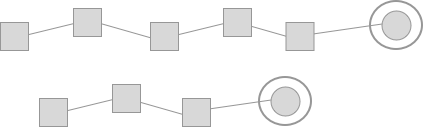
\includegraphics[scale=0.3]{img/exe-feed}
%   \end{center}

\begin{center}
\begin{tabular}{lcl}
$\Delta \ \Lambda^0$         &:& $\times^0$ \\
$\Delta \ \Lambda^{n}$       &:& $\Lambda^{n-1}$ \\
\end{tabular}
\end{center}


\newpage
  \subsubsection*{Лямбда числення}

Для розробки нашої теорії ми застосуємо інтуітіоністську теорію типів Мартіна Льофа.
Ця система типів буде застосовуватися для довення робочих теорем. База мови складає
лябмда числення як внутрішня мова декартово-замкненої категорії. Лямбда числення в своїй
основі скаладається з конструктора типу яка визначає функції та елімінатора -- аплікації
функції до аргументу.

\begingroup
\parbox[t][][l]{0.40\textwidth}{

\begin{prooftree}
\AxiomC{$\Gamma\ x:A \vdash\ B$ }
\UnaryInfC{$\Gamma \vdash fun\ x : A \rightarrow B$}
\end{prooftree}

}
\hspace{0.1cm}
\parbox[t][][r]{0.60\textwidth}{

\begin{prooftree}
\AxiomC{$\Gamma\ f:A \rightarrow B$ }
\AxiomC{$\Gamma\ a:A$ }
\BinaryInfC{$\Gamma \vdash f \ a : B$}
\end{prooftree}

}
\endgroup

  \subsubsection*{Алегбраїчні типи даних}

Далі йде внутрішня мова алгебраїчних типів даних яка складається з суми та добутку,
за допомогою яких контруюються суми-протоколи та кортежі-пакети, а також {\bf nil} типу-атому,
яким зручно термінувати рекурсивні типи даних, такі як {\bf cons}.

\begin{prooftree}
\AxiomC{}
\UnaryInfC{$\Gamma \vdash\ \bot$ }
\end{prooftree}

\begingroup
\parbox[t][][l]{0.40\textwidth}{

\begin{prooftree}
\AxiomC{$\Gamma \vdash\  a:A$ }
\AxiomC{$\Gamma \vdash\  b:B$ }
\BinaryInfC{$\Gamma \vdash\  (a,b) : A \times B$ }
\end{prooftree}

\begin{prooftree}
\AxiomC{$\Gamma \vdash\  a:A$ }
\AxiomC{$\Gamma \vdash\  b:B$ }
\BinaryInfC{$\Gamma\vdash a\ |\ b : A \otimes B$}
\end{prooftree}

}
\hspace{0.1cm}
\parbox[t][][r]{0.60\textwidth}{


\begin{prooftree}
\AxiomC{$\Gamma\ x: A \times B$ }
\UnaryInfC{$\Gamma \vdash fst\ x : A$;
           $\Gamma \vdash snd\ x : B$}
\end{prooftree}

\begin{prooftree}
\AxiomC{$\Gamma\ x: A \otimes B$ }
\UnaryInfC{$\Gamma \vdash inl\ x : A$;
           $\Gamma \vdash inr\ x : B$}
\end{prooftree}


}
\endgroup


  \subsubsection*{Процеси і протоколи}

Також ми анонсуємо процес як фундаменльний тип даних, подібний до функції але який здатний
тритати певний стан у вигляді типа коротежа та бути здатним реагувати на повідомлення суми.

\begin{prooftree}
\AxiomC{$\Gamma\ \vdash \Sigma, X$ }
\AxiomC{$\Gamma\ \vdash a : \Sigma \times X \rightarrow X$ }
\BinaryInfC{$\Gamma \vdash {proc}_{\Sigma}\ a : \pi $}
\end{prooftree}

\begin{prooftree}
\AxiomC{$\Gamma\ \vdash proc : \pi$ }
\AxiomC{$\Gamma\ \vdash m : \Sigma$ }
\BinaryInfC{$\Gamma \vdash {join}_{\Sigma}\ (m, proc) \rightarrow \Sigma$;
            $\Gamma \vdash {async}_{\Sigma}\ (m, proc) \rightarrow \Sigma$}
\end{prooftree}

  \subsubsection*{Типи процесів}

\begin{center}
\begin{tabular}{lll}
         $action$ &:& ${proc}_{Proc}\ (Proc\ |\ \Sigma) \times process \rightarrow process$ \\
         $event$  &:& ${proc}_{App}\ (App\ |\ \Sigma) \times cx \rightarrow cx$ \\
         $add$    &:& ${proc}_{Store}\ (Store\ |\ \Sigma) \times container \rightarrow container$ \\
\end{tabular}
\end{center}

\newpage

  \subsubsection*{Логіка та квантори}

Далі йдуть квантори $\forall$ та $\exists$ які теж виражаються як конструкції типів:

\begingroup
\parbox[t][][l]{0.40\textwidth}{

\begin{prooftree}
\AxiomC{$\Gamma\ x: A \vdash B$ }
\AxiomC{$\Gamma\ \vdash A$ }
\BinaryInfC{$\Gamma\ \vdash \Pi (x : A) B $}
\end{prooftree}

\begin{prooftree}
\AxiomC{$\Gamma\ x: A \vdash B$ }
\AxiomC{$\Gamma\ \vdash A$ }
\BinaryInfC{$\Gamma\ \vdash \Sigma (x : A) B $}
\end{prooftree}

}
\hspace{0.1cm}
\parbox[t][][r]{0.60\textwidth}{

\begin{prooftree}
\AxiomC{$\Gamma\ \vdash a : A$ }
\AxiomC{$\Gamma\ x : A \vdash B$ }
\AxiomC{$\Gamma\ b : B (x=a)$ }
\TrinaryInfC{$\Gamma\ \vdash (a,b) : \Pi (x : A) B $}
\end{prooftree}


\begin{prooftree}
\AxiomC{$\Gamma\ \vdash a : A$ }
\AxiomC{$\Gamma\ x : A \vdash B$ }
\AxiomC{$\Gamma\ b : B (x=a)$ }
\TrinaryInfC{$\Gamma\ \vdash (a,b) : \Sigma (x : A) B $}
\end{prooftree}

}
\endgroup

\begingroup
\parbox[t][][l]{0.40\textwidth}{

\begin{prooftree}
\AxiomC{$\Gamma\ \vdash x: A$ }
\AxiomC{$\Gamma\ \vdash x': A$ }
\BinaryInfC{$\Gamma\ \vdash Id_A (x,x')$}
\end{prooftree}

}
\hspace{0.1cm}
\parbox[t][][r]{0.60\textwidth}{

\begin{center}
\begin{tabular}{lll}
рефлексивність &:& $Id_A(a,a)$ \\
пістановка &:& $Id_A(a,a') \rightarrow B(x=a) \rightarrow B(x=a')$ \\
%симетричність &:& $Id_A(a,b) \rightarrow Id_A(b,a)$  \\
%транзитивність &:& $Id_A(a,b) \rightarrow Id_A(b,c) \rightarrow Id_A(a,c)$ \\
%конгруентність &:& $(f: A \rightarrow B) \rightarrow Id_A(x,x') \rightarrow Id_B(f(x),f(x'))$ \\
\end{tabular}
\end{center}
}\endgroup



  \subsubsection*{Типи категорії}

\begin{center}
\begin{tabular}{lll}
           $store^3$ &:& $\times^3 \Lambda_{id_seq}\ \Lambda_{table}\ \Lambda_{feed}$ \\
          $roster^2$ &:& $\times^2 \Lambda_{feed}\ \Lambda^2_{feed}$ \\
             $app^2$ &:& $\times^2 \Lambda_{session}\ \Lambda_{proc}$ \\
           $depot^1$ &:& $\times^1 \Lambda_{account}$ \\
             $act^1$ &:& $\times^1 \Lambda_{proc}$ \\
\end{tabular}
\end{center}

  \subsubsection*{Контраваріантні процеси}

  Ко-процеси це моноїди з перевернутою стрілкою, які визначають зворотній шлях виконання
  події та обернену зміни стану в зворотньому порядку. З точки зоро типів нічого не змінюється,
  однак оберненої функції-фунтора процесу-моноїда може і не існувати. Процеси які є
  одночасно коваріантними та контраваріантними називаються інваріантними процесами, сигнатура яких
  алгебраїчно збігається з сигнатурою бінарного дерева.

\begin{center}
\begin{tabular}{lcl}
$X$         &:& $\times^{i}$ \\
$\Lambda$   &:& $\times^{4} \ I \ X \ \Lambda_{next} \ \Lambda_{prev}$ \\
            &|& $\bot$ \\
\end{tabular}
\end{center}

\begin{center}
$st(p) = p(st-1)$ — застосування функції до протокольної заявки та стану процесу
$p-1(st) = st-1$ — обернена функція
\end{center}

  \subsubsection*{Суми процесів}

  Віртуальне середовище виконує моноїдальні процеси як одну велику суму.
  Кожна така сума представляє собою віртуальну одиницю виконання -- віртуальну машину.

\newpage

   \subsubsection*{Модель віртуального середовища}

\begin{figure}[h!]
\centering
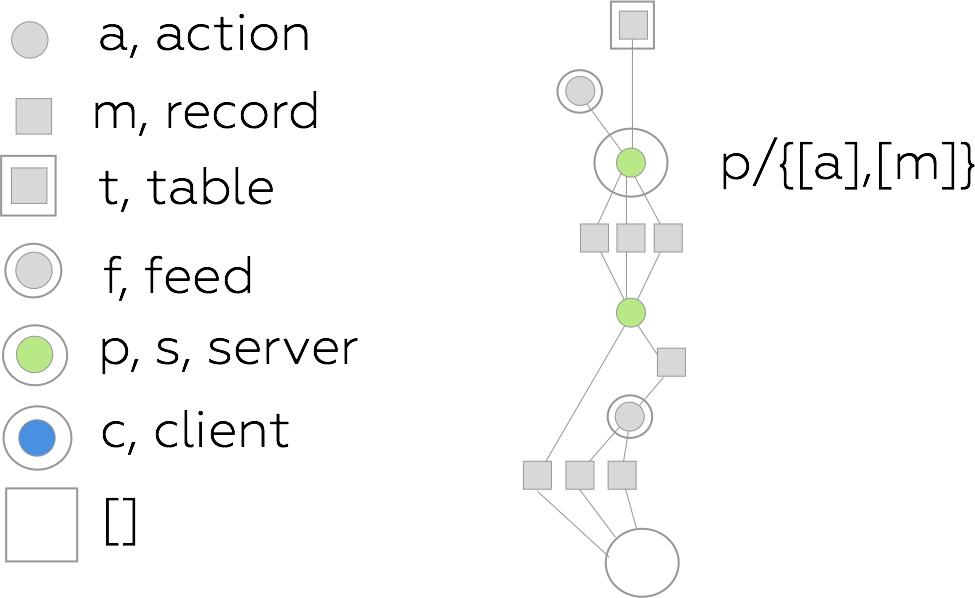
\includegraphics[scale=0.3]{img/exe-legend}
\caption{Базові елементи віртуального середовища}
\end{figure}

\subsection*{Віртуальна машина}

{\bf action} is the piece of code applied to message using pattern matching.\\
{\bf record} is the tuple that defines a protocol.\\
{\bf client} is the true customer of the system who is using service on daily basis.\\
{\bf server} is the process nicely scheduled by the system.\\
{\bf feed} is the server managed list of records.\\
{\bf table} is the ixset or ets based queryable tables.\\

\subsection*{Обчислювальні категорії}

{\bf app} is the web clients monoidal state machine.\\
{\bf proc} is the oriented graph monoidal executional engine.\\
{\bf store} is the 2-category key-value database.\\

\newpage
\subsection{Завдання дослідження}
\vspace{0.5cm}
   Тактична мета даної роботи -- це
   реалізація усіх верхніх компонентів OSI на базі метамоделі Exe на мові Erlang.
   Побудова зручної сучасної гнучкої верифікованої теорії
   з компактною системою типів є основним завданням даного дослідження.

   \begin{center}
   \vspace{1cm}
   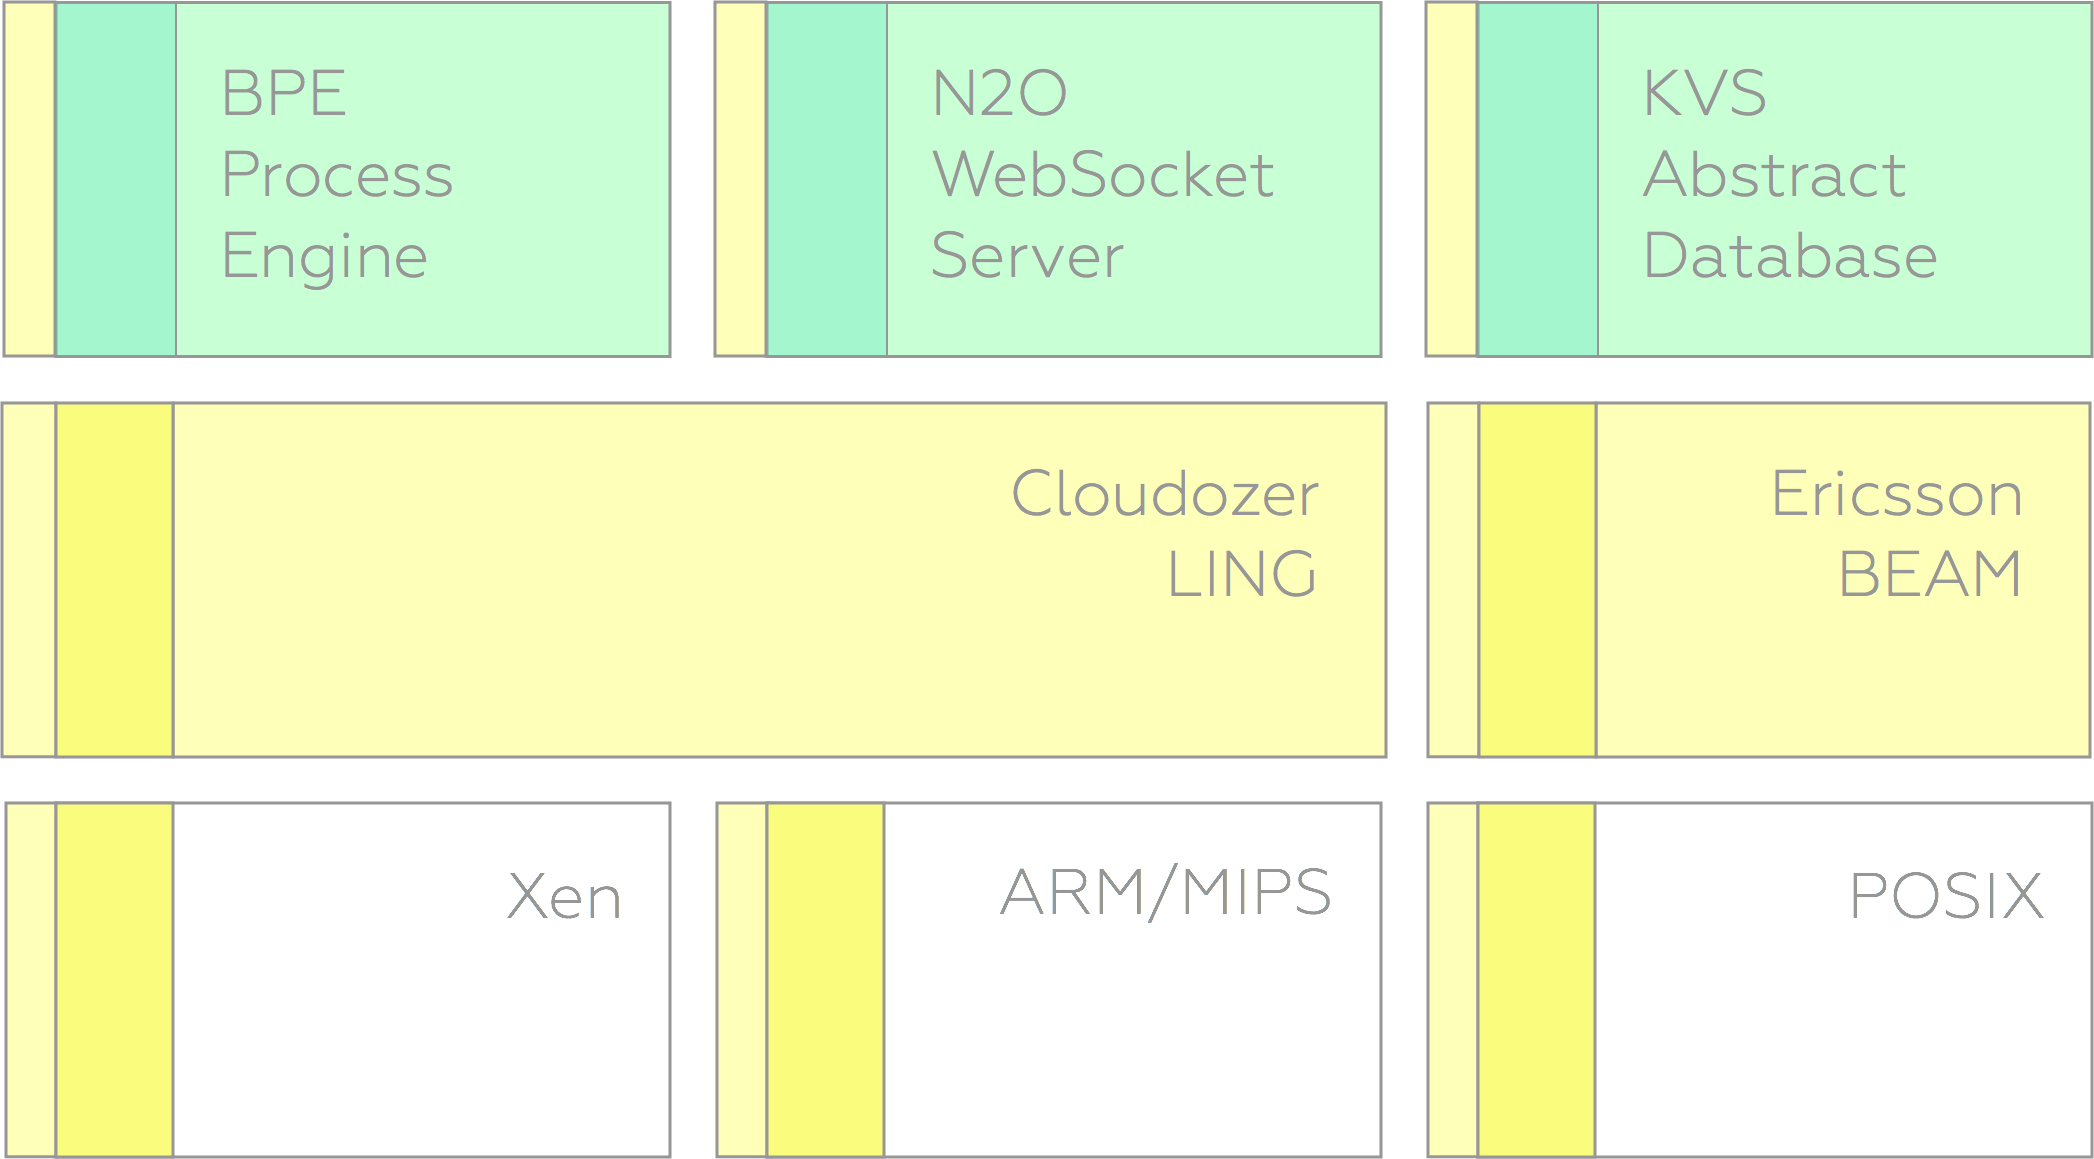
\includegraphics[scale=0.15]{img/exe-res}
   \end{center}

\newpage
\subsection{Мета дослідження}
\vspace{0.5cm}
   Основною метою дослідження є збезпечення виконання критеріїв відповідності
   показників ефективності, детермінованості та якості шляхом впровадження
   результату даної теорії, комплексу програмного забезпечення у виробничий процес.

   За рахунок компактності передбачається значна економія складності та простота у експлуатації,
   що веде до сниження собівартості впровадження. Коректність передбачає заміну
   автоматозаваному тестуванню, а закритість середовища дозволяє гнучко використовувати
   середовище на різних виробничих платформах.
   \\

\subsection{Результати}
\vspace{0.5cm}
   Одна з останніх систем, яка була впроваджена для заміни існуючої системи, мала
   показники у співвідношенні розміру 10, швидкості 20 та виконання 3. Інші системи
   у історичній послідовності мали ці показники такими 10, 2, 8, та 19, 5, 5.
   В середньому показники ефективності відрізняються більше ніж на пів порядка
   в кращу сторону після впровадження продуктів на базі розробленої моделі.
   Існують продукти також і на інших мовах програмування.

\newpage
\begin{thebibliography}{9}

\bibitem{}         Per Martin-Löf \textit{Intuitionistic Type Theory} 1984
\bibitem{erl}      J.Armstrong. \textit{Making reliable distributed systems in the presence of sodware errors} 2003.
\bibitem{comm}     Robin Milner. \textit{ A Calculus of Communicating Systems.} 1986.
\bibitem{lawvere1} William Lawvere. \textit{Conceptual Mathematics.} 1997.
\bibitem{pierce}   Benjamin Pierce. \textit{Basic category theory for computer scientist.} 2004.
\bibitem{mclane}   Сандерс Мак Лейн. \textit{Категории для работающего математика.} 2004.
\bibitem{tla}      Leslie Lamport. \textit{Specifying Systems} 2004.
\bibitem{barr1}    Michael Barr and Charles Wells. \textit{Toposes, Triples and Theories.} 2000.
\bibitem{barr2}    Michael Barr and Charles Wells. \textit{Category Theory for Computing Science.} 1995.
\bibitem{bakur}    И.Бакур, А.Деляну. \textit{Введение в теорию категори и функторов} 1972.
\bibitem{commpi}   Robin Milner. \textit{Communicating and Mobile Systems: The $\pi$-calculus.} 1999.
\bibitem{polypi}   Robin Milner. \textit{The Polyadic $\pi$-Calculus: A Tutorial.} 1993.
\bibitem{mass}     Коваленко. \textit{Теория Массового Обслуживания.} 1965.
\bibitem{meseguer} Meseguer, Montanari.  \textit{Petri Nets Are Monoids} 1990.
\bibitem{}         D.Mostrous, V.Vasconcelos \textit{Session Typing for a Featherweight Erlang} 1990.
\bibitem{}         S.Marlow, P.Wadler \textit{A practical subtyping system for Erlang} 1997
\bibitem{}         Philip Wadler \textit{Call-by-Value is Dual to Call-by-Name} 1000
\end{thebibliography}

\vspace{3\baselineskip}
\paragraph{}
З повагою, команда Synrc.
\paragraph{}
\vspace{3\baselineskip}
\begin{tabular}{ll}
        & Сохацький Максим, технічний директор \\
        & Кирилов Володимир, співзасновник
\end{tabular}


\end{document}
